%! TeX root = ../../main.tex

\chapter{Model and methods}

\section{Hubbard model}

In this work we use the Hubbard model \cite{Hubbard1997} to describe strongly correlated systems.
Denoting the creator of site $i$ and spin $\sigma\in\{\uparrow,\downarrow\}$
as $d^\dag_{i\sigma}$ and respective annihilator as $d_{i\sigma}$ its Hamiltonian reads
\begin{equation}
    H
    =
    -t\sum_{\langle i j\rangle\sigma}
    (d^\dag_{i\sigma} d^{\pdag}_{j\sigma} + d^\dag_{j\sigma} d^{\pdag}_{i\sigma})
    +
    U\sum_i n_{i\uparrow} n_{i\downarrow}
    +
    (\epsilon - \mu)\sum_{i\sigma} n_{i\sigma},
\end{equation}
with a sketch given in \zcref{fig:hubbard-model}.
Each site can be occupied by up to two electrons.
The first term describes the kinetics of the system:
Electrons can hop between nearest-neighbors $\langle i j\rangle$
defining the hopping amplitude $t$.
If two electrons are on the same site, they are repulsed by the Coulomb interaction $U$
expressed by the second term (occupation $n_{i\sigma} = d^\dag_{i\sigma} d^{\pdag}_{i\sigma}$).
The last term describes the on-site energy $\epsilon$ and
chemical potential $\mu$ as we are in the grand canonical ensemble.

\begin{figure}[ht]
    \centering
    %! TeX root = ../../main.tex
% chktex-file 8

\def\nsites{3}
\def\len{3mm}
\def\wdth{3mm}
\def\lwdth{0.75mm}
\def\spinsep{0.1}

\newcommand\nup[2]
{
    \draw [red, {Latex[length=\len, width=\wdth]}-, line width=\lwdth]
    ({#2*2}, {0.6-#1*2}) -- ({#2*2}, {-0.6-#1*2});
}

\newcommand\ndn[2]
{
\draw [blue, -{Latex[length=\len, width=\wdth]}, line width=\lwdth]
({#2*2}, {0.6-#1*2}) -- ({#2*2}, {-0.6-#1*2});
}

\newcommand\nupdn[2]
{
\draw [red, {Latex[length=\len, width=\wdth]}-, line width=\lwdth]
({#2*2-\spinsep}, {0.6-#1*2}) -- ({#2*2-\spinsep}, {-0.6-#1*2});
\draw [blue, -{Latex[length=\len, width=\wdth]}, line width=\lwdth]
({#2*2+\spinsep},{0.6-#1*2}) -- ({#2*2+\spinsep},{-0.6-#1*2});
\node at ({#2*2+0.5},{-#1*2+0.5}) {$U$};
}

\newcommand\hoppingdown[2]{
    \draw [->, thick]
    ({#2*2-0.4}, {-0.4-#1*2}) to [bend right=30] node[midway, left] {$t$} ({#2*2-0.4}, {-1.6-#1*2});
}

\newcommand\hoppingright[2]{
    \draw [->, thick]
    ({#2*2+0.4}, {0.4-#1*2}) to [bend left=30] node[midway, above] {$t$} ({#2*2+1.6}, {0.4-#1*2});
}

\begin{tikzpicture}
    [
        node distance=10mm,
        inner sep=1mm,
        minimum size=5mm,
        site/.style={rectangle,draw=black,very thick,fill=gray!20},
    ]
    % grid
    \draw [dashed] (1,-1) grid[step=20mm] (2*\nsites+1,-2*\nsites-1);
    % sites
    \foreach \x in {1,...,\nsites}
        {
            \foreach \y in {1,...,\nsites}
                {
                    % \node [site, label=\x\y] at (2*\x,-2*\y) (s\x\y) {};
                    \node [site] at (2*\x,-2*\y) (s\x\y) {};
                }
        }
    % add electrons
    \nup{1}{1}
    \ndn{1}{2}
    \nupdn{1}{3}
    \ndn{2}{3}
    \nup{3}{1}
    \nupdn{3}{2}
    \hoppingdown{1}{1}
    \hoppingright{1}{1}
\end{tikzpicture}

    \caption{
        Hubbard model on a 2D square lattice.
        $t$ denotes hopping between nearest-neighbors,
        while $U$ describes the Coulomb repulsion on a doubly occupied site.
    }
    \label{fig:hubbard-model}
\end{figure}

Although the model looks simple, no analytical solution in arbitrary dimension exists.
The problem is that the kinetic part is diagonal in momentum space,
while the Coulomb interaction is diagonal in real space.
Thus, in DMFT (details in TODO) we instead solve a simpler model which has only one correlated site.
% TODO: reference DMFT

\section{Anderson impurity model}
\label{sec:anderson-impurity-model}

The Hamiltonian of the Anderson impurity model \cite{Anderson1961} can be split into
an interacting and non-interacting part
\begin{equation}
    H = H_0 + H_\mathrm{int}.
    \label{eq:impurity-Hamiltonian}
\end{equation}
Denoting the impurity (labeled $i$) annihilators by $d_\sigma$
and bath (labeled $b$) annihilators by $b_{k\sigma}$
it can be written as
\begin{align}
    H_0
     & =
    (\epsilon - \mu) \sum_{\pk\sigma} n_\sigma
    +
    \sum_{k\sigma} \epsilon_{k\sigma}^{\pdag} b^\dag_{k\sigma} b^{\pdag}_{k\sigma}
    +
    \sum_{k\sigma} \left(V^{\ps}_{k\sigma} d^\dag_{\pk\sigma} b^{\pdag}_{k\sigma}
    + V_{j\sigma}^* b^\dag_{k\sigma} d^{\pdag}_{\pk\sigma} \right),
    \\
    H_\mathrm{int}
     & =
    U n_\uparrow n_\downarrow.
    \label{eq:anderson-interaction}
\end{align}
Here,
$\epsilon$ denotes the impurity energy,
$\mu$ the chemical potential,
$n_\sigma = d^\dag_\sigma d^{\pdag}_\sigma$ the impurity occupation,
$\epsilon_{k\sigma}$ the energy levels of the bath,
and $V_{k\sigma}$ the hybridization between the bath and impurity.
A graphical representation of this \emph{star geometry} is given in \zcref{subfig:geometry-star}:
each bath site has a given filling
and electrons from each bath site can hop in and out of the impurity.

\begin{figure}[ht]
    \centering
    \savebox{\imagebox}{%! TeX root = ../../main.tex

\begin{tikzpicture}
    [
        node distance=2mm,
    ]
    % draw sites
    \foreach \i [remember=\i as \lasti, evaluate=\i as \filling using -0.1*\i+0.9] in {1,...,7}
        {
            \ifnum\i=1
                \node [bath={\filling}, label=right:$l_\i$] (l\i) {};
            \else
                \node [bath={\filling}, label=right:$l_\i$] (l\i) [above=of l\lasti] {};
            \fi
        }
    \node [impurity={0.5}, label=left:$i$] (impurity) [left=5mm of l4] {};

    % connect sites
    \foreach \i in {1,...,7}
        {
            \draw (impurity.east) to [out=0,in=180,looseness=0.3] (l\i.west);
        }
\end{tikzpicture}
} % save for height alignment
    \begin{subfigure}{0.45\textwidth}
        \centering
        \usebox{\imagebox}
        \caption{star geometry}
        \label{subfig:geometry-star}
    \end{subfigure}
    \begin{subfigure}{0.45\textwidth}
        \centering
        \raisebox{\dimexpr0.5\ht\imagebox-0.5\height}
        {
            %! TeX root = ../../main.tex

\begin{tikzpicture}[
        node distance=2mm,
    ]
    % draw sites
    \node [impurity={0.5}, label=left:$i$] (impurity) {};
    \node [bath={0.5}, label=right:$b$] (mirror) [right=of impurity] {};
    \foreach \i [remember=\i as \lasti] in {1,...,3}
        {
            \ifnum\i=1
                \node [bath={1.0}, label=below:$v_1$] (v\i) [below=of mirror] {};
                \node [bath={0.0}, label=above:$c_1$] (c\i) [above=of mirror] {};
            \else
                \node [bath={1.0}, label=below:$v_\i$] (v\i) [right=of v\lasti] {};
                \node [bath={0.0}, label=above:$c_\i$] (c\i) [right=of c\lasti] {};
            \fi
        }

    % connect sites
    \draw (impurity.east) to (mirror.west);
    \draw (impurity.south) to [out=270,in=180] (v1.west);
    \draw (impurity.north) to [out=90,in=180] (c1.west);
    \draw (mirror.south) to (v1.north);
    \draw (mirror.north) to (c1.south);
    \foreach \i [remember=\i as \lasti (initially 1)] in {2,...,3}
        {
            \draw (v\lasti.east) -- (v\i.west);
            \draw (c\lasti.east) -- (c\i.west);
        }
\end{tikzpicture}

        }
        \caption{natural impurity orbitals}
        \label{subfig:geometry-natural-impurity-orbitals}
    \end{subfigure}
    \caption{
        Anderson impurity model in different geometries.
        Impurity (square) interacting with bath sites (circles).
        Site occupation is indicated by fill level,
        where a full site corresponds to double occupation.
        Furthermore, hopping between sites is shown by lines.
        \subref{subfig:geometry-star} is the conventional \emph{star geometry};
        \subref{subfig:geometry-natural-impurity-orbitals} the \emph{natural impurity orbitals}
        are explained in \zcref{sec:natural-impurity-orbitals}
        (adapted from~\cite{Lu2019}).
    }
\end{figure}

\subsection{Natural impurity orbitals}
\label{sec:natural-impurity-orbitals}

To solve the Anderson impurity model,
we can use Slater determinants to decompose the wave function
\begin{equation}
    \ket{\psi} = \sum_{i=1}^M \alpha_i \ket{\phi_i}
\end{equation}
using any orthonormal set of basis functions.
With the occupation number,
we can express the number of electrons in each spin sector as
\begin{equation}
    n_\sigma = n_{i,\sigma} + \sum_{k=1}^N n_{b,k\sigma}.
\end{equation}
For a fixed amount of electrons $n_\uparrow + n_\downarrow$ on $N$ bath sites and the impurity,
a combination of
\begin{equation}
    M = \binom{N+1}{n_\uparrow} \cdot \binom{N+1}{n_\downarrow}
\end{equation}
determinants are necessary to fully describe the wave function.
For a half-filled system ($n_\uparrow = n_\downarrow = (N+1)/2$)
with $N+1=140$ sites, this is approximately $\num{9e81}$
exceeding the number of protons in the observable universe $\bigO{\num{e80}}$. % Eddington number
As this is not treatable numerically,
we need to truncate a certain number of determinants with the smallest probabilities.
To save computational resources,
we want to find a new basis in which the probabilities decay faster than those of the star geometry
(further details in \cite{Bi2019}).

A commonly employed basis set in quantum chemistry are the \emph{natural orbitals}
in which the ground state density is diagonal.
However,
a naive implementation of the natural orbitals will inevitably mix the original impurity
and bath sites transforming the local Coulomb interaction (\zcref{eq:anderson-interaction})
among multiple new sites,
losing locality \cite{Lu2014,Lu2019}.
We therefore use the \emph{natural impurity orbitals}
which only rotates bath orbitals while keeping the impurity untouched.
This new geometry is shown in \zcref{subfig:geometry-natural-impurity-orbitals}.
The unchanged impurity $i$ is connected to a mirror site (labeled $m$) and two chains.
Following the convention of \cite{Lu2014,Lu2019},
we call sites in the almost fully filled chain valence bath sites (labeled $v$),
and sites in the almost empty chain as conduction bath sites (labeled $c$).
Hopping between sites is again shown by lines.

\section{Configuration interaction}
\label{sec:configuration-interaction}

\question{Difference configuration interaction vs.\ restricted active space?}

Using the natural impurity orbitals (\zcref{sec:natural-impurity-orbitals}) allows us to
write the ground state in a basis which has optimal scaling behavior with respect to
the number of bath sites \cite{Lu2019}.
However, the computational complexity still grows combinatorial with each added bath site.
To alleviate the scaling problem we employ the same method as \citeauthor{Lu2019} \cite{Lu2019}
which is sketched in \zcref{fig:aim-separation}.

\begin{figure}[ht]
    \centering
    %! TeX root = ../../main.tex

\begin{tikzpicture}[
        inner sep=1mm,
        node distance=4mm,
    ]
    % sites
    \node [impurity={0.5}] (impurity) {};
    \node [bath={0.5}] (mirror) [right=of impurity] {};
    \foreach \i [remember=\i as \lasti] in {1,...,6}
        {
            \ifnum\i=1
                \node [bath={0.85}] (v\i) [below=of mirror] {};
                \node [bath={0.15}] (c\i) [above=of mirror] {};
            \else
                \ifnum\i=2
                    \node [bath={0.9}] (v\i) [right=of v\lasti] {};
                    \node [bath={0.1}] (c\i) [right=of c\lasti] {};
                \else
                    \ifnum\i=4
                        \node [bath={1.0}] (v\i) [right=8mm of v\lasti] {};
                        \node [bath={0.0}] (c\i) [right=8mm of c\lasti] {};
                    \else
                        \node [bath={1.0}] (v\i) [right=of v\lasti] {};
                        \node [bath={0.0}] (c\i) [right=of c\lasti] {};
                    \fi
                \fi
            \fi
        }

    % labels (separate node for box fit below)
    \node (impuritylabel)[left=0mm of impurity] {$i$};
    \node (mirrorlabel)[right=0mm of mirror] {$m$};
    \node (v1label)[below=0mm of v1] {$v_1$};
    \node (v3label)[below=0mm of v3] {$v_{L\vphantom{+1}}$}; % phantom for bounding box size
    \node (v4label)[below=0mm of v4] {$v_{L+1}$};
    \node (c1label)[above=0mm of c1] {$c_1$};
    \node (c3label)[above=0mm of c3] {$c_{L\vphantom{+1}}$}; % phantom for bounding box size
    \node (c4label)[above=0mm of c4] {$c_{L+1}$};


    % connect sites
    \draw (impurity.east) to (mirror.west);
    \draw (impurity.south) to [out=270,in=180] (v1.west);
    \draw (impurity.north) to [out=90,in=180] (c1.west);
    \draw (mirror.south) to (v1.north);
    \draw (mirror.north) to (c1.south);
    \foreach \i [remember=\i as \lasti (initially 1)] in {2,...,6}
        {
            \draw (v\lasti.east) -- (v\i.west);
            \draw (c\lasti.east) -- (c\i.west);
        }

    % bounding box
    \node [
        draw,
        rectangle,
        rounded corners,
        line width=0.2pt,
        fit=(impuritylabel) (v3label) (c3label),
        label=left:$|\phi_I\rangle$,
    ] {};
    \node [
        draw,
        rectangle,
        rounded corners,
        line width=0.2pt,
        fit=(v4label) (v6) (c4label) (c6),
        label=right:$|\phi_{II}\rangle$,
    ] {};
\end{tikzpicture}

    \caption{
        Separation of the wave function into two components
        $\ket{\phi_I}$ and $\ket{\phi_{II}}$ denoted by two boxes.
    }
    \label{fig:aim-separation}
\end{figure}

The full Hilbert space is projected onto a subspace that only contains
empty conduction sites $\ket{\mathbb{0}_c}$
and full valence sites $\ket{\mathbb{1}_v}$ for $l>L$.
The ground state can be written as
\begin{equation}
    \ket{\psi_0}
    =
    \ket{\phi_I} \otimes \ket{\mathbb{0}_c} \otimes \ket{\mathbb{1}_v}
    =
    \ket{\phi_I} \otimes \ket{\phi_{II}},
\end{equation}
where $\ket{\phi_I}$ is the exact ground state calculated by ED for some $L\ll N/2$
($N/2$ chain length at half-filling)
and $\ket{\phi_{II}} = \ket{\mathbb{0}_c} \otimes \ket{\mathbb{1}_v}$ is a reference state.

In the next step we loosen the restriction of empty conduction and full valence bath sites.
The $p=1$ projection allows one state to differ from the reference state:
Either one electron of $\ket{\phi_I}$ enters the empty conduction sites
or one electron from the full valence sites enters $\ket{\phi_I}$.
In the $p=2$ projection two states are allowed to differ.
This allows the following possibilities for $\ket{\phi_{II}}$:
\begin{itemize}
    \item two electrons in the conduction bath sites $c_l$ ($l\ge L$)
    \item two holes in the valence bath sites $v_l$ ($l\ge L$)
    \item one electron in the conduction bath sites $c_l$
          and one hole in the valence bath sites $v_l$ ($l\ge L$)
\end{itemize}

\section{Lanczos algorithm}
\label{sec:lanczos-algorithm}

The Lanczos algorithm \cite{Lanczos1950} can be used to approximate the extremal eigenvalues
of a hermitian $n\times n$ matrix.
In our case we are interested in the ground state and low energy excitations of a
given Hamiltonian $H$.
The method is especially useful if $H$ is sparse and too large to decompose fully.
It is based on a Krylov basis
\begin{equation}
    \mathcal{K}^M(H, \vec{q}) = \spn\{\vec{q}, H\vec{q}, H^2\vec{q}, \ldots, H^{M-1}\vec{q}\}
\end{equation}
for a given vector $\vec{q}$.
Typically, the value $M$ is very small compared to the matrix size: $M \ll n$.
Instead of a simple power iteration, the Lanczos algorithm is described by the
following recurrence relation
\begin{equation}
    b_j\vec{q}_{j+1} = H\vec{q}_j - a_j\vec{q}_j - b_{j-1}\vec{q}_{j-1}
    \label{eq:Lanczos-recurrence}
\end{equation}
with a normalized starting vector $\vec{q}_1$ and $\vec{q}_0 = \vec{0}$.
The coefficients are chosen such that each Lanczos vector $\vec{q}_j$ is orthonormal to each other
\begin{equation}
    a_j = \vec{q}_j^\dag H \vec{q}_j,
    \qquad
    b_j = \vec{q}_{j+1}^\dag H \vec{q}_j.
\end{equation}
For numerical stability \cite{Paige1972, Paige1976}
we instead calculate the coefficients as
\begin{equation}
    a_j = \vec{v}_j^\dag(H \vec{v}_j - \beta_{j-1}\vec{v}_{j-1}),
    \qquad
    b_j = \norm{H\vec{v}_j - \alpha\vec{v}_j -  \beta_{j-1}\vec{v}_{j-1}}.
\end{equation}
From this relation we can create the tridiagonal matrix
\begin{equation}
    T
    =
    \begin{pmatrix}
        a_1 & b_1 &        &         &         \\
        b_1 & a_2 & b_2    &         &         \\
            & b_2 & a_3    & \ddots  &         \\
            &     & \ddots & \ddots  & b_{M-1} \\
            &     &        & b_{M-1} & a_M
    \end{pmatrix}
    \label{eq:tridiagonal-scalar}
\end{equation}
and matrix collecting all Lanczos vectors
\begin{equation}
    Q = (\vec{q}_1, \vec{q}_2, \ldots, \vec{q}_M).
\end{equation}
Then, \zcref{eq:Lanczos-recurrence} in matrix form can be rewritten as
\begin{equation}
    H Q = Q T + b_{M}\vec{q}_{M+1}\vec{e}_{M}^\top,
\end{equation}
where $\vec{e}_M$ is the Euclidean basis vector with $M$-th component 1 and all other 0.
Rearranging gives
\begin{equation}
    T = Q^\dag H Q,
\end{equation}
which means that $T$ is the orthogonal projection of $H$ onto
the subspace $\mathcal{K}^M(H, \vec{q}_1)$ \cite{Cullum1985}.

\subsection{Block Lanczos}

Instead of calculating only one vector $\vec{q}_j$ in each step,
one can calculate $p$ vectors simultaneously.
We define
\begin{equation}
    Q_1 = (\vec{q}_1^{(1)}, \vec{q}_1^{(2)}, \ldots, \vec{q}_1^{(p)})
\end{equation}
to be an $n\times p$ orthonormal block of starting vectors
and $Q_0 = \mathbb{0}_{n\times q}$.
Then the recurrence relation (\zcref{eq:Lanczos-recurrence}) can be rewritten as
\begin{equation}
    Q_{j+1} B_j = H Q_j - Q_j A_j - Q_{j-1} B_{j-1}^\dag,
    \label{eq:block-Lanczos-recurrence}
\end{equation}
with $A_j$, $B_j$ matrices of size $p\times p$ chosen such that each block $Q_j$ is orthonormal
to each other.
The block tridiagonal matrix of size $Mp\times Mp$ is written as
\begin{equation}
    T
    =
    \begin{pmatrix}
        A_1 & B_1^\dag &          &         &              \\
        B_1 & A_2      & B_2^\dag &         &              \\
            & B_2      & A_3      & \ddots  &              \\
            &          & \ddots   & \ddots  & B_{M-1}^\dag \\
            &          &          & B_{M-1} & A_M
    \end{pmatrix}.
    \label{eq:tridiagonal-block}
\end{equation}
For the calculation for $B_j$ one needs to orthornormalize
\begin{equation}
    \tilde Q_{j+1} = H Q_j - Q_j A_j - Q_{j-1} B_{j-1}^\dag,
\end{equation}
which is not unique.
For instance, a QR decomposition $Q_{j+1} B_j = \tilde Q_{j+1}$
results in an upper triangular matrix $B_j$ which gives $T$ a compactly banded structure
\cite{Cullum1985, Golub2013}.
In our work however, we use symmetric Löwdin orthonormalization \cite{Lowdin1950, Brass2021}
which is based on the singular value decomposition
$\tilde Q_{j+1} = U_{j+1} \Sigma_{j+1} V_{j+1}^\dag$.
We define the overlap matrix as
\begin{equation}
    S_{j+1} \coloneqq \tilde Q_{j+1}^\dag \tilde Q_{j+1} = V_{j+1} \Sigma_{j+1}^2 V_{j+1}^\dagger
\end{equation}
and its roots as
\begin{equation}
    S_{j+1}^{1/2}  = V_{j+1} \Sigma_{j+1} V_{j+1}^\dagger,
    \qquad
    S_{j+1}^{-1/2} = V_{j+1} \Sigma_{j+1}^{-1} V_{j+1}^\dagger.
\end{equation}
The resulting vectors are then
\begin{align}
    Q_{j+1} & = \tilde Q_{j+1} S_{j+1}^{-1/2} \qquad \text{and} \\
    B_j     & = S_{j+1}^{1/2}.
\end{align}
We use this method as it guarantees hermiticity in the off-diagonal blocks $B_j^\dag = B_j$
albeit losing the compactly banded structure for $T$.
If $\tilde Q_j$ is rank-deficient,
this method can still be applied \cite{Brass2021} by only inverting the block of
non-vanishing singular values
\begin{equation}
    \Sigma =
    \begin{pmatrix}
        \Sigma_i \neq 0 & 0 \\
        0               & 0
    \end{pmatrix}
    \qquad
    \Sigma^{-1} =
    \begin{pmatrix}
        \Sigma_i^{-1} & 0 \\
        0             & 0
    \end{pmatrix},
\end{equation}
still guaranteeing orthonormality against previous states $Q_i^\dag Q_j = \mathbb{0}_{q\times q}$
for $i \in \{1,\ldots,j-1\}$ \cite{Golub2013}.

\section{Correlators}
\label{sec:correlators}

The retarded correlator for two fermionic operators $A, B$ is defined as
\begin{align}
    C(t) = -\mi \Theta(t) \expval{\acomm{A(t)}{B}},
\end{align}
with the step function $\Theta$ and anticommutator $\acomm{\cdot}{\cdot}$.
$A(t) = \me^{\mi H t} A \me^{-\mi H t}$ is given in the Heisenberg picture.
At zero temperature $T=0$, the expectation value is evaluated on the ground state
$\expval{\,\cdot\,} = \sandwich{\psi_0}{\,\cdot\,}{\psi_0}$ only.
Following the notation of \cite{Bulla1998,Kugler2022},
we will denote the Fourier transform $\mathcal{F}$ as
\begin{equation}
    C_\omega
    =
    \mathcal{F}[C(t)]
    \coloneq
    \lim_{\delta\to0^+}
    \int_{-\infty}^\infty\! \md t\> \me^{\mi (\omega + \mi\delta) t} C(t)
    \eqcolon
    \dangle{A}{B}{\omega}.
\end{equation}
Furthermore,
we split this expression into two components $C_\omega = C^+_\omega + C^-_\omega$ with
\begin{subequations}
    \begin{align}
        C^+_\omega
         & =
        \expval*{A \frac{1}{\omega + \mi0^+ - H + E_0} B}
        =
        \sum_n \frac{\sandwich{\psi_0}{A}{n}\sandwich{n}{B}{\psi_0}}{\omega + \mi0^+ - E_n + E_0}, \\
        C^-_\omega
         & =
        \expval*{B \frac{1}{\omega + \mi0^+ + H - E_0} A}
        =
        \sum_n \frac{\sandwich{\psi_0}{B}{n}\sandwich{n}{A}{\psi_0}}{\omega + \mi0^+ + E_n - E_0}.
    \end{align}
\end{subequations}
The sum is over a complete basis $H\ket{n} = E_n\ket{n}$ with ground state energy $E_0$.
A derivation is given in \zcref{app:fourier-transform}.
The problem however is the exponential algorithmic complexity:
For $N$ sites (bath and impurity), the number of all possible states scales as $O(4^N)$
limiting exact diagonalization (ED) to $N=O(10)$ sites.

For the choice $A=d_\sigma, B=d_\sigma^\dag$ the correlator describes
the propagation of an electron/hole in the system and is called Green's function $G_\omega$.

\subsection{Representation}

Using the Lanczos algorithm we can represent correlators as the first component of the inverse
of our (block) tridiagonal matrix $T$ \cite{Lu2014}, see \zcref{eq:tridiagonal-scalar,eq:tridiagonal-block}

\begin{subequations}
    \begin{align}
        C_\omega
         & =
        \frac{b_0^2}{\omega + \mi0^+ - a_1 - \frac{b_1^2}{\omega + \mi0^+ - a_2 - \ldots}}
        \qquad
         &
         & \text{(scalar)},                                                                         \\
        C_\omega
         & = B_0\frac{1}{\omega + \mi0^+ - A_1 - B_1\frac{1}{\omega + \mi0^+ - A_2 - \ldots}B_1}B_0
        \qquad
         &
         & \text{(block)}.
    \end{align}
\end{subequations}
In the block case $\frac{1}{D} \wedgeq D^{-1}$ is meant as the matrix inverse
and $\omega + \mi0^+ \wedgeq (\omega + \mi0^+)\mathbb{1}$ a shorthand notation
for a diagonal matrix.
The value(s) $b_0$ ($B_0$) normalize the initial state(s) of
the (block) Lanczos routine respectively.
In contrast to \texttt{QUANTY} \cite{Ackermann2024} we always keep our matrices $B_i$ hermitian,
even if they are rank-deficient.
We will call this the \emph{continued fraction} representation.

Diagonalizing $T$ gives us a sum of poles instead:
\begin{subequations}
    \begin{align}
        C_\omega
         & =
        \sum_{i=1}^M \frac{w_i}{\omega + \mi0^+ - \epsilon_i}
        \label{eq:correlator-sum}
        \qquad
         &   & \text{(scalar)}, \\
        C_\omega
         & =
        \sum_{i=1}^M \frac{W_i}{\omega + \mi0^+ - \epsilon_i}
        \qquad
         &   & \text{(block)}.
    \end{align}
\end{subequations}
In order for these correlators to represent physical quantities,
the weights $w_i$ must be non-negative in the scalar case
and $W_i$ positive semidefinite in the block case.

Only diagonalizing from the second part of $T$ onwards gives us the \emph{Anderson representation}
\begin{subequations}
    \begin{align}
        C_\omega
         & =
        \frac{b_0^2}{\omega + \mi0^+ - a_1 - \sum_{j=2}^M \frac{w_j}{\omega + \mi0^+ - \epsilon_j}}
        \qquad
         &
         &
        \text{(scalar)},                                                                                   \\
        C_\omega
         & = B_0\frac{1}{\omega + \mi0^+ - A_1 - \sum_{j=2}^M \frac{W_j}{\omega + \mi0^+ - \epsilon_j}}B_0
        \qquad
         &
         &
        \text{(block)}.
        \label{eq:correlator-anderson-block}
    \end{align}
\end{subequations}
A detailed explanation on how to switch between these representations is given in \cite{Lu2014}.

\subsection{Broadening and spectra}

Given a correlator $C_\omega$ the corresponding spectral part is defined as
\begin{equation}
    A_\omega \coloneq -\frac{1}{\muppi}\Im C_\omega,
\end{equation}
which is easy to calculate if it is given as a sum of poles \zcref{eq:correlator-sum}:
\begin{equation}
    A_\omega = \sum_{i=1}^m w_i \delta(\omega - \epsilon_i).
    \label{eq:spectral-sum}
\end{equation}
The real and imaginary part of a correlator are not independent
but related by Kramers-Kronig transformations (Hilbert transform)
\begin{subequations}
    \begin{align}
        \Re C_\omega
         & =
        - \frac{1}{\muppi} \mathcal{P}\! \int_{-\infty}^\infty\! \md\omega'
        \frac{\Im C_{\omega'}}{\omega - \omega'}
        \label{eq:kramers-kroneg-real} \\
        \Im C_\omega
         & =
        \phantom{-} \frac{1}{\muppi} \mathcal{P}\! \int_{-\infty}^\infty\! \md\omega'
        \frac{\Re C_{\omega'}}{\omega - \omega'}.
        \label{eq:kramers-kronig-imag}
    \end{align}
\end{subequations}

Thus, we can broaden our delta-peaks from \zcref{eq:spectral-sum}
for the imaginary part and obtain the real part through \zcref{eq:kramers-kroneg-real}.
We will denote the broadened correlator as $C_z$
to contrast it to $C_\omega$, which has no broadening.
In this work we will use the following three schemes:
\begin{enumerate}[(i)]
    \item Lorentzian broadening characterized by $\delta$:
          \label{item:lorentzian}
          \begin{equation}
              \delta(\omega - \omega_0)
              \longrightarrow
              \frac{1}{\muppi}\frac{\delta}{(\omega - \omega_0)^2 + \delta^2}
          \end{equation}
    \item Gaussian broadening characterized by $\sigma$:
          \label{item:gaussian}
          \begin{equation}
              \delta(\omega - \omega_0)
              \longrightarrow
              \frac{1}{\sqrt{2\muppi \sigma^2}}\exp\left(-\frac{(\omega - \omega_0)^2}{2\sigma^2}\right)
          \end{equation}
    \item logarithmic Gaussian characterized by $b$ \cite{Bulla2008}:
          \label{item:logarithmic-gaussian}
          \begin{equation}
              \delta(\omega - \omega_0)
              \longrightarrow
              \Theta(\omega\omega_0)\frac{\me^{-b^2/4}}{b\omega_0\sqrt{\muppi}}\exp\left(-\frac{(\ln\omega-\ln\omega_0)^2}{b^2}\right)
          \end{equation}
\end{enumerate}

\begin{figure}[ht]
    \centering
    %! TeX root = ../../main.tex

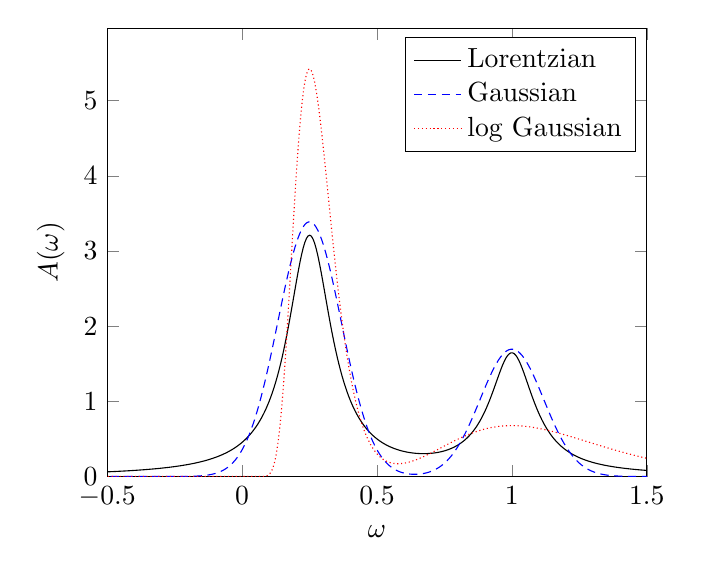
\begin{tikzpicture}
    \begin{axis}
        [
            xlabel=$\omega$,
            ylabel=$A(\omega)$,
            xmin=-0.5,
            xmax=1.5,
            ymin=0,
            legend cell align=left,
        ]

        % weight and locations of two poles
        \def\L{0.25}
        \def\W{1.0}
        \def\LL{1.0}
        \def\WW{0.5}

        % Lorentzian
        \def\DELTA{0.1}
        \addplot [color=black, domain=-1:2, samples=500] { \DELTA/pi*(\W/((x-\L)^2 + \DELTA^2) + \WW/((x-\LL)^2 + \DELTA^2))};
        \addlegendentry{Lorentzian}

        % Gaussian
        \def\SIGMA{0.11774100225154747} % HWHM sqrt(2*ln(2))*\DELTA
        \addplot [color=blue, densely dashed, domain=-1:2, samples=500] { 1/sqrt(2*pi*\SIGMA^2)*(\W*exp(-(x-\L)^2 / 2/ \SIGMA^2) + \WW*exp(-(x-\LL)^2 / 2 / \SIGMA^2))};
        \addlegendentry{Gaussian}

        % logarithmic Gaussian
        \def\B{0.4}
        \addplot [color=red, densely dotted, domain=-1:2, samples=900] { x > 0 ? exp(-\B^2 / 4) / (\B*sqrt(pi)) * (\W / \L *exp(-ln(x/\L)^2 / \B^2) + \WW / \LL *exp(-ln(x/\LL)^2 / \B^2)) : 0 };
        \addlegendentry{log Gaussian}
    \end{axis}
\end{tikzpicture}

    \caption{
        Plot of the spectral part of a correlator
        $C_\omega = \frac{1}{\omega + \mi0^+ - 0.25} + \frac{0.5}{\omega + \mi0^+ - 1}$
        using Lorentzian, Gaussian, and logarithmic Gaussian broadening.
    }
    \label{fig:broadening}
\end{figure}

A comparison of these broadenings is given in \zcref{fig:broadening}.
The Lorentzian and Gaussian spectra consist of symmetric peaks
with the former decaying slower compared to the latter.
The peaks generated by the logarithmic Gaussian are asymmetric
and sharper if the pole is closer to $\omega=0$.
As all poles are at located at $\omega>0$,
the spectrum of the log Gaussian vanishes for $\omega\le0$.

\section{Self-energy}
\label{sec:self-energy}

As mentioned in the previous section,
the Green's function $G_\omega$ describes the propagation of an electron/hole in our system.
If our system is non-interacting ($U=0$ in \zcref{eq:anderson-interaction}),
we call it the non-interacting Green's function $G_{0, \omega}$.
The quantity that connects these two objects is the self-energy defined by the Dyson equation
\begin{equation}
    \Sigma_\omega = (G_{0, \omega})^{-1} - (G_\omega)^{-1}.
    \label{eq:dyson}
\end{equation}

In \cite{Lu2014},
this equation was used to represent the self-energy by the constant Hartree term $\Sigma^\mH$
and a sum of poles
\begin{equation}
    \Sigma_\omega = \Sigma^\mH + \sum_j \frac{w_j}{\omega + \mi0^+ - \epsilon_j}.
    \label{eq:self-energy-sum-of-poles}
\end{equation}
For the self-energy to be physical, all weights must be positive.
On a system with finite bath sites and floating-point arithmetic however,
this was violated and poles with negative weight had to be merged into neighbors
such that only positive weight remained.

Therefore, we calculate the self-energy using the symmetric improved estimator
$\Sigma^\mIFG_\omega$ \cite{Kugler2022}
which will be summarized in the following:
We introduce the auxiliary operator
\begin{equation}
    q_\sigma = \comm{d_\sigma}{H_\mathrm{int}}
\end{equation}
for the Anderson impurity model (\zcref{sec:anderson-impurity-model}),
allowing us to calculate the Hartree term directly
\begin{equation}
    \Sigma^\mH = \expval{\acomm{q^\dag_\sigma}{d^{\pdag}_\sigma}}.
\end{equation}
We then employ a quadratic shift
\begin{equation}
    \tilde q_\sigma = q_\sigma - \Sigma^\mH d_\sigma
    \label{eq:quadratic-shift}
\end{equation}
and obtain four correlation functions
\begin{subequations}
    \begin{alignat}{2}
        G_\omega
         & =
        \dangle{d^{\pdag}_\sigma}{d_{\sigma}^\dag}{\omega},
         &
        \qquad
        I_\omega
         & =
        \dangle{\tilde q^{\pdag}_\sigma}{\tilde q_{\sigma}^\dag}{\omega} \\
        F^\mL_\omega
         & =
        \dangle{\tilde q^{\pdag}_\sigma}{d_{\sigma}^\dag}{\omega},
         &
        \qquad
        F^\mR_\omega
         & =
        \dangle{d^{\pdag}_\sigma}{\tilde q_{\sigma}^\dag}{\omega}.
    \end{alignat}
\end{subequations}
The self-energy is computed as
\begin{equation}
    \Sigma^\mIFG_\omega
    =
    \Sigma^\mH + I_\omega - F^\mL_\omega (G_\omega)^{-1} F^\mR_\omega.
\end{equation}
Concretely, we first calculate the components of our block correlator as
\begin{subequations}
    \begin{align}
        C^+_\omega
         & =
        \sandwich*
        {\psi_0}
        {
            \begin{pmatrix}
                \tilde q^{\pdag}_\sigma \\
                d^{\pdag}_\sigma
            \end{pmatrix}
            \frac{1}{\omega + \mi0^+ - H + E_0}
            \begin{pmatrix}
                \tilde q^\dag_\sigma & d^\dag_\sigma
            \end{pmatrix}
        }
        {\psi_0}
        =
        \begin{pmatrix}
            I^+_\omega      & F^{\mL+}_\omega \\
            F^{\mR+}_\omega & G^+_\omega
        \end{pmatrix} \\
        C^-_\omega
         & =
        \sandwich*
        {\psi_0}
        {
            \begin{pmatrix}
                \tilde q^\dag_\sigma \\
                d^\dag_\sigma
            \end{pmatrix}
            \frac{1}{\omega + \mi0^+ + H - E_0}
            \begin{pmatrix}
                \tilde q^{\pdag}_\sigma & d^{\pdag}_\sigma
            \end{pmatrix}
        }
        {\psi_0}
        =
        \begin{pmatrix}
            I^-_\omega      & F^{\mR-}_\omega \\
            F^{\mL-}_\omega & G^-_\omega
        \end{pmatrix}
    \end{align}
\end{subequations}
and add them together
\begin{equation}
    C_\omega
    =
    C^+_\omega + (C^-_\omega)^\top
    =
    \begin{pmatrix}
        I_\omega       & F^{\mL}_\omega \\
        F^{\mR}_\omega & G_\omega
    \end{pmatrix}.
\end{equation}
In \cite{Kugler2022} it was noted that $F^{\mR}_\omega = (F^{\mL}_\omega)^\dag$
might be violated numerically.
We do not have this problem as hermiticity is enforced on $C_\omega$.

Given each correlator as a sum of poles, \citeauthor{Kugler2022} \cite{Kugler2022} broadened
each correlator and calculated the broadened self-energy $\Sigma_z$.
In this work we instead calculate the self-energy on the real axis
using the Schur complement \cite{Schur1917}
\todo{credit Aleksandrs} %TODO: credit Aleksandrs
\begin{equation}
    \Sigma_\omega = \Sigma^\mH + \left([(C_\omega)^{-1}]_{11}\right)^{-1}.
\end{equation}
To invert our block correlation function, we first bring it to
the Anderson representation (\zcref{eq:correlator-anderson-block}):
\begin{equation}
    C_\omega = B\frac{1}{\omega + \mi0^+ - A - D_\omega}B,
\end{equation}
with matrices $A$, $B$ and a block sum of poles $D_\omega$.
The scaling matrix $B$ contains the square root of the zeroth moments,
e.g.\ its first element $B_{11} = U/2$ at half-filling.
Due to the quadratic shift (\zcref{eq:quadratic-shift}), it is diagonal.
The Schur complement is then
\begin{equation}
    \left([(C_\omega)^{-1}]_{11}\right)^{-1}
    =
    (B)_{11} \frac{1}{\omega + \mi0^+ - (A)_{11} - (D_\omega)_{11}} (B)_{11}.
\end{equation}
Diagonalizing this expression gives us the self-energy in the same form as
\zcref{eq:self-energy-sum-of-poles}.
Contrasting against \zcref{eq:dyson},
all pole weights are positive by construction
and no merging of negative weight into neighbors is necessary.

\section{Ground state}

In order to calculate correlators and expectation values listed in
\zcref{sec:correlators, sec:self-energy} at $T=0$,
one first needs to obtain the ground state of a given impurity Hamiltonian $H$
(\zcref{eq:impurity-Hamiltonian}).
As an initial guess we take the state with all valence bath sites $v_k$ filled in combination with
a singlet state in the impurity $i$ and mirror site $m$
(the filling of each site is sketched in \zcref{subfig:geometry-natural-impurity-orbitals}):
\begin{equation}
    \ket*{\psi_0^{(1)}}
    =
    \frac{1}{\sqrt{2}}
    \left(d^\dag_\uparrow m^\dag_\downarrow - d^\dag_\downarrow m^\dag_\uparrow\right)
    \prod_{k\sigma} v^\dag_{k\sigma}
    \ket{0}.
\end{equation}
Given this state, we can calculate an approximate ground state energy
\begin{equation}
    E_0^{(1)} = \sandwich*{\psi_0^{(1)}}{H}{\psi_0^{(1)}}
\end{equation}
and variance
\begin{equation}
    \var^{(1)}
    =
    \sandwich*{\psi_0^{(1)}}{\left(H - E_0^{(1)}\right)^2}{\psi_0^{(1)}}.
\end{equation}
As this approximation is not sufficient for calculations,
we employ the Lanczos method (\zcref{sec:lanczos-algorithm}) with restarting
as described in \cite{Lu2014}:
Given an approximate ground state $\ket{\psi_0^{(i)}}$,
we calculate a new Krylov basis $\mathcal{K}^5(H, \ket{\psi_0^{(i)}}$ which is diagonalized.
From this, we calculate a new state $\ket{\psi_0^{(i+1)}}$
with a new ground state energy $E_0^{(i+1)}$
and variance $\var^{(i+1)}$.
This loop is repeated until the variance falls below a given tolerance
as it must vanish for a true eigenstate of $H$.

One should note that even if the variance is exactly zero for a state $\ket{\tilde\psi_0}$
in the CI approximation (\zcref{sec:configuration-interaction}),
this state is not a true eigenstate of the unrestricted Hamiltonian.
Applying $H$ on $\ket{\tilde\psi_0}$ without any restriction
will generate new states \cite{Lu2014}.
It is just that these state have (hopefully) such small weight allowing us to ignore them.

\section{DMFT}

Hybridization function
\begin{align}
    \Delta_\omega = \sum_{k\sigma} \frac{\abs{V_{k\sigma}}^2}{\omega - \epsilon_{k\sigma}}
\end{align}

\section{Bethe lattice}
